\documentclass[11pt]{article}
\usepackage[review]{acl}
\usepackage{times}
\usepackage{latexsym}
\usepackage[T1]{fontenc}
\usepackage[utf8]{inputenc}
\usepackage{microtype}
\usepackage{inconsolata}
\usepackage{booktabs}
\usepackage{graphicx}

% Generated from results/paper_stats.json; do not edit.
\newcommand{\DiagnosticSlices}{87}
\newcommand{\DiagnosticFlagged}{14}
\newcommand{\DiagnosticInconclusive}{9}
\newcommand{\DiagnosticRows}{87,000}
\newcommand{\DiagnosticThreshold}{0.50}
\newcommand{\RewardModelName}{xlm-roberta-base}
\newcommand{\RewardTrainRows}{50,000}
\newcommand{\RewardDevRows}{5,000}
\newcommand{\RewardSteps}{500}
\newcommand{\RewardCheckpointSeeds}{1}
\newcommand{\PrimaryPool}{18}
\newcommand{\PrimarySegments}{410}
\newcommand{\ExternalPool}{30}
\newcommand{\ExternalSegments}{541}
\newcommand{\PoolPermutations}{100}
\newcommand{\BanditContexts}{541}
\newcommand{\BanditActions}{30}
\newcommand{\BanditTrainContexts}{367}
\newcommand{\BanditTestContexts}{174}
\newcommand{\BanditTestDocuments}{56}
\newcommand{\BanditUpdates}{200}
\newcommand{\BanditSeeds}{5}
\newcommand{\UniformCesa}{66.27}
\newcommand{\WMTPrimaryName}{WMT25}
\newcommand{\WMTExternalName}{WMT26}
\newcommand{\AllExcludedSlices}{0}
\newcommand{\AllRemovedRows}{0}
\newcommand{\AllDevSpearman}{0.438}
\newcommand{\AllPrimaryFull}{-7.86}
\newcommand{\AllPrimaryChange}{-0.58}
\newcommand{\AllExternalFull}{44.70}
\newcommand{\AllExternalChange}{-19.66}
\newcommand{\AllBanditCesa}{33.07}
\newcommand{\AllBanditChange}{-33.19}
\newcommand{\AllBanditLow}{-43.39}
\newcommand{\AllBanditHigh}{-21.39}
\newcommand{\AllTopProbability}{0.734}
\newcommand{\FilteredExcludedSlices}{14}
\newcommand{\FilteredRemovedRows}{239,364}
\newcommand{\FilteredDevSpearman}{0.449}
\newcommand{\FilteredPrimaryFull}{-7.47}
\newcommand{\FilteredPrimaryChange}{-0.20}
\newcommand{\FilteredExternalFull}{46.37}
\newcommand{\FilteredExternalChange}{-17.99}
\newcommand{\FilteredBanditCesa}{33.86}
\newcommand{\FilteredBanditChange}{-32.40}
\newcommand{\FilteredBanditLow}{-43.44}
\newcommand{\FilteredBanditHigh}{-19.88}
\newcommand{\FilteredTopProbability}{0.695}
\newcommand{\RandomExcludedSlices}{14}
\newcommand{\RandomRemovedRows}{235,497}
\newcommand{\RandomDevSpearman}{0.432}
\newcommand{\RandomPrimaryFull}{-7.79}
\newcommand{\RandomPrimaryChange}{-0.52}
\newcommand{\RandomExternalFull}{46.43}
\newcommand{\RandomExternalChange}{-17.93}
\newcommand{\RandomBanditCesa}{39.67}
\newcommand{\RandomBanditChange}{-26.60}
\newcommand{\RandomBanditLow}{-36.34}
\newcommand{\RandomBanditHigh}{-15.22}
\newcommand{\RandomTopProbability}{0.564}
\newcommand{\DirectionExcludedSlices}{14}
\newcommand{\DirectionRemovedRows}{247,332}
\newcommand{\DirectionDevSpearman}{0.434}
\newcommand{\DirectionPrimaryFull}{-7.61}
\newcommand{\DirectionPrimaryChange}{-0.33}
\newcommand{\DirectionExternalFull}{48.04}
\newcommand{\DirectionExternalChange}{-16.32}
\newcommand{\DirectionBanditCesa}{67.92}
\newcommand{\DirectionBanditChange}{+1.66}
\newcommand{\DirectionBanditLow}{+1.23}
\newcommand{\DirectionBanditHigh}{+2.10}
\newcommand{\DirectionTopProbability}{0.056}
\newcommand{\FilteredMinusAllPrimary}{+0.39}
\newcommand{\FilteredMinusAllPrimaryLow}{-0.41}
\newcommand{\FilteredMinusAllPrimaryHigh}{+1.25}
\newcommand{\FilteredMinusAllExternal}{+1.67}
\newcommand{\FilteredMinusAllExternalLow}{+0.01}
\newcommand{\FilteredMinusAllExternalHigh}{+3.42}
\newcommand{\FilteredMinusRandomPrimary}{+0.32}
\newcommand{\FilteredMinusRandomPrimaryLow}{-0.43}
\newcommand{\FilteredMinusRandomPrimaryHigh}{+1.10}
\newcommand{\FilteredMinusRandomExternal}{-0.06}
\newcommand{\FilteredMinusRandomExternalLow}{-1.86}
\newcommand{\FilteredMinusRandomExternalHigh}{+1.75}
\newcommand{\FilteredMinusDirectionPrimary}{+0.14}
\newcommand{\FilteredMinusDirectionPrimaryLow}{-0.54}
\newcommand{\FilteredMinusDirectionPrimaryHigh}{+0.85}
\newcommand{\FilteredMinusDirectionExternal}{-1.67}
\newcommand{\FilteredMinusDirectionExternalLow}{-3.69}
\newcommand{\FilteredMinusDirectionExternalHigh}{+0.32}


\title{Optimizing What the Labels Teach: Auditing Machine Translation Rewards under Metric--Annotation Disagreement}

\author{Anonymous ACL submission}

\begin{document}
\maketitle

\begin{abstract}
Learned machine translation rewards inherit the strengths and artifacts of
their human training labels.  Motivated by AmanaMT's finding that apparent
metric failures can reflect annotation protocol, we ask whether removing
dataset slices with strong metric--annotation disagreement makes rewards more
reliable under optimization.  We train otherwise matched reward models on all
available direct-assessment labels, after targeted slice exclusion, and after
two matched-removal controls.  Increasing best-of-$N$ pressure lowers held-out
human quality for every reward on both expert MQM and cESA candidate pools.
Targeted filtering sometimes improves over the all-data reward but does not
reliably beat matched removal.  In a finite-action contextual bandit, exact
policy-gradient optimization of three rewards sharply reduces held-out cESA;
a direction-matched reward instead remains diffuse and slightly improves it.
Mechanism analysis shows that the failing policies learn strong preferences
for one translation system.  The results establish reward overoptimization
and sensitivity to reward-training composition, but not disagreement filtering
as a remedy.  We release an exactly checkable bandit implementation and
source-traced paper statistics.
\end{abstract}

\section{Introduction}

Machine translation metrics increasingly serve as rewards for reranking and
reinforcement learning.  Optimizing an imperfect proxy can increase predicted
reward while decreasing the desired outcome \citep{gao-etal-2023-scaling}, and
this failure has been demonstrated directly for translation quality-estimation
rewards \citep{he-etal-2024-improving}.  A reward's training labels are one
possible source of the mismatch.

AmanaMT reported large variation in metric--human agreement across translation
directions \citep{thompson-2026-amanamt}.  Subsequent auditing found that some
of this pattern aligns with changes in annotation protocol.  Expert MQM can
produce different conclusions from crowd ratings \citep{freitag-etal-2021-experts},
and the shared-task organizers explicitly cautioned against segment-level use
of reference-based direct assessment \citep{freitag-etal-2022-results}.

We turn that diagnosis into a falsifiable intervention: remove language-pair
by year slices where two automatic metrics agree much more strongly with each
other than one agrees with direct-assessment labels.  We ask whether this
targeted removal produces rewards that retain human quality under increasing
optimization pressure, beyond simply training on fewer labels.

Our answer is negative but informative.  All learned rewards exhibit offline
overoptimization.  The targeted condition does not consistently outperform
matched controls, while an earlier-year direction-matched control behaves very
differently during policy optimization.  This shifts the conclusion from
``bad labels can be detected and removed'' to a narrower one: reward behavior
is highly sensitive to training-data composition, and the present diagnostic
does not identify a sufficient correction.

\section{Metric--annotation disagreement}

For each language-pair by year slice, we define
\begin{equation}
D = \rho(\textsc{Comet},\textsc{Bleurt})
  - \rho(\textsc{Comet},\textsc{DA}),
\end{equation}
where $\rho$ is segment-level Spearman agreement.  This is a disagreement
diagnostic, not proof that an individual annotation is incorrect: COMET and
BLEURT may share preferences or training overlap.

The frozen audit covers \DiagnosticSlices{} slices and \DiagnosticRows{}
sampled annotations.  We flag a slice only when the lower paired-bootstrap
endpoint for $D$ exceeds \DiagnosticThreshold{}.  This flags
\DiagnosticFlagged{} slices; \DiagnosticInconclusive{} additional slices cross
the threshold and remain included.  The threshold predates reward training and
the held-out evaluations.

\section{Reward models and controls}

We fine-tune \RewardModelName{} regressors with identical initialization
procedure and budgets.  Every condition uses \RewardTrainRows{} sampled
training rows, \RewardDevRows{} common development rows, and \RewardSteps{}
updates.  Human holdout outcomes do not affect checkpoint selection.

\begin{table}[t]
\centering
\small
\setlength{\tabcolsep}{5pt}
\begin{tabular}{lrrr}
\toprule
Reward data & Slices & Source rows & Dev $\rho$ \\
\midrule
All data & \AllExcludedSlices & \AllRemovedRows & \AllDevSpearman \\
Disagreement-filtered & \FilteredExcludedSlices & \FilteredRemovedRows & \FilteredDevSpearman \\
Size-matched random & \RandomExcludedSlices & \RandomRemovedRows & \RandomDevSpearman \\
Direction/year matched & \DirectionExcludedSlices & \DirectionRemovedRows & \DirectionDevSpearman \\
\bottomrule
\end{tabular}
\caption{Frozen reward-training conditions.  ``Source rows'' is removal from
the eligible DA pool before equal-size training samples are drawn.}
\label{tab:conditions}
\end{table}

The size-matched random control removes retained-clear slices with similar
total volume.  The direction-matched sensitivity removes earlier, retained
into-English slices because no retained-clear slices exist in the flagged
later-year strata.  It therefore changes year as well as label composition.
Only \RewardCheckpointSeeds{} reward checkpoint exists per condition; policy
seeds below do not measure reward-model training variability.

\section{Offline optimization pressure}

We apply best-of-$N$ selection to fixed candidate sets.  Candidate order is
randomized \PoolPermutations{} times per source and shared across rewards.
The primary \WMTPrimaryName{} holdout contains \PrimarySegments{} segments,
expert MQM outcomes, and up to \PrimaryPool{} candidates.  The external
\WMTExternalName{} holdout contains \ExternalSegments{} Chinese--Japanese
segments, cESA outcomes, and \ExternalPool{} machine-system candidates; the
released human-postedited output is excluded.

\begin{figure}[t]
\centering
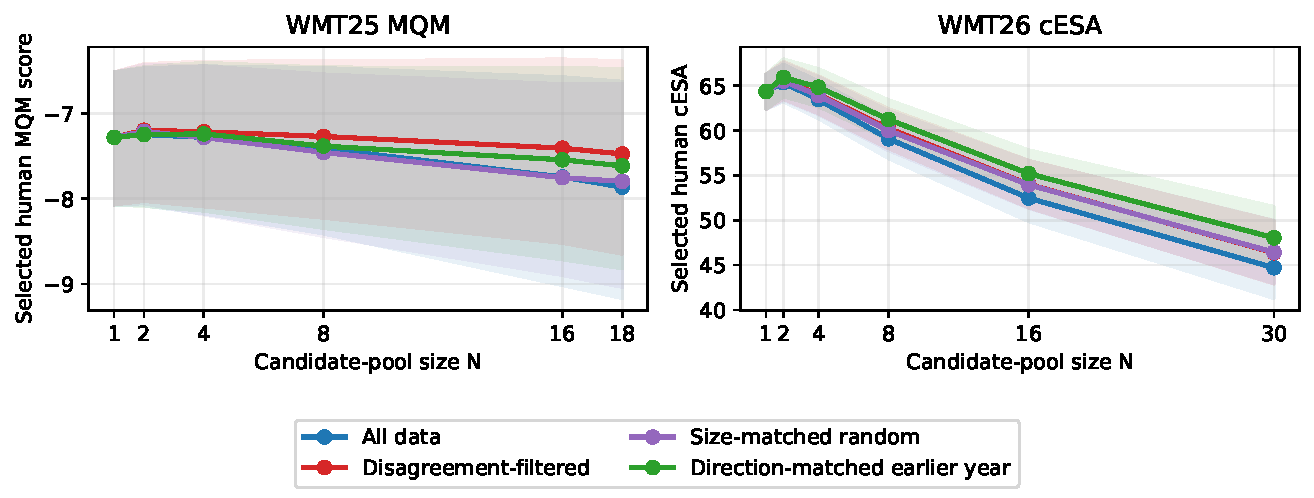
\includegraphics[width=\linewidth]{figures/best_of_n.pdf}
\caption{Held-out human quality as candidate-pool size increases.  Bands are
paired bootstrap intervals.  Higher is better in both panels.}
\label{fig:bestofn}
\end{figure}

\begin{table}[t]
\centering
\small
\setlength{\tabcolsep}{3.5pt}
\begin{tabular}{lrrrr}
\toprule
& \multicolumn{2}{c}{\WMTPrimaryName{} MQM} &
\multicolumn{2}{c}{\WMTExternalName{} cESA} \\
Reward & Full & $\Delta$ & Full & $\Delta$ \\
\midrule
All & \AllPrimaryFull & \AllPrimaryChange & \AllExternalFull & \AllExternalChange \\
Filtered & \FilteredPrimaryFull & \FilteredPrimaryChange & \FilteredExternalFull & \FilteredExternalChange \\
Random & \RandomPrimaryFull & \RandomPrimaryChange & \RandomExternalFull & \RandomExternalChange \\
Direction/year & \DirectionPrimaryFull & \DirectionPrimaryChange & \DirectionExternalFull & \DirectionExternalChange \\
\bottomrule
\end{tabular}
\caption{Full-pool human quality and its change from single-candidate
selection.  Negative changes indicate reward overoptimization.}
\label{tab:bestofn}
\end{table}

Figure~\ref{fig:bestofn} and Table~\ref{tab:bestofn} show deterioration for
every reward and endpoint.  At full pressure, disagreement filtering differs
from all-data selection by \FilteredMinusAllPrimary{}
$[\FilteredMinusAllPrimaryLow,\FilteredMinusAllPrimaryHigh]$ on the primary
holdout and \FilteredMinusAllExternal{}
$[\FilteredMinusAllExternalLow,\FilteredMinusAllExternalHigh]$ externally.
However, it differs from size-matched random removal by
\FilteredMinusRandomPrimary{}
$[\FilteredMinusRandomPrimaryLow,\FilteredMinusRandomPrimaryHigh]$ and
\FilteredMinusRandomExternal{}
$[\FilteredMinusRandomExternalLow,\FilteredMinusRandomExternalHigh]$.
Thus the external improvement over all data does not establish a targeted
filtering advantage over removing comparable volume.

\section{Exactly checkable policy optimization}

We next use the external candidate set as a contextual bandit.  Source segments
are contexts and machine systems are actions, following prior work on bandit
system selection \citep{naradowsky-etal-2020-machine}.  The policy uses hashed
source-character features, domain indicators, and a logit for each system.
Documents are split before fitting: \BanditTrainContexts{} contexts train the
policy and \BanditTestContexts{} contexts from \BanditTestDocuments{} documents
are held out.  Human cESA is never used for learning or stopping.

The finite action space permits exact expected-reward gradients.  We compare
that reference with ordinary one-action REINFORCE across \BanditSeeds{} policy
seeds for \BanditUpdates{} updates.  Independent reconstruction from saved
action probabilities verifies the reported proxy reward, cESA, and entropy.

\begin{figure*}[t]
\centering
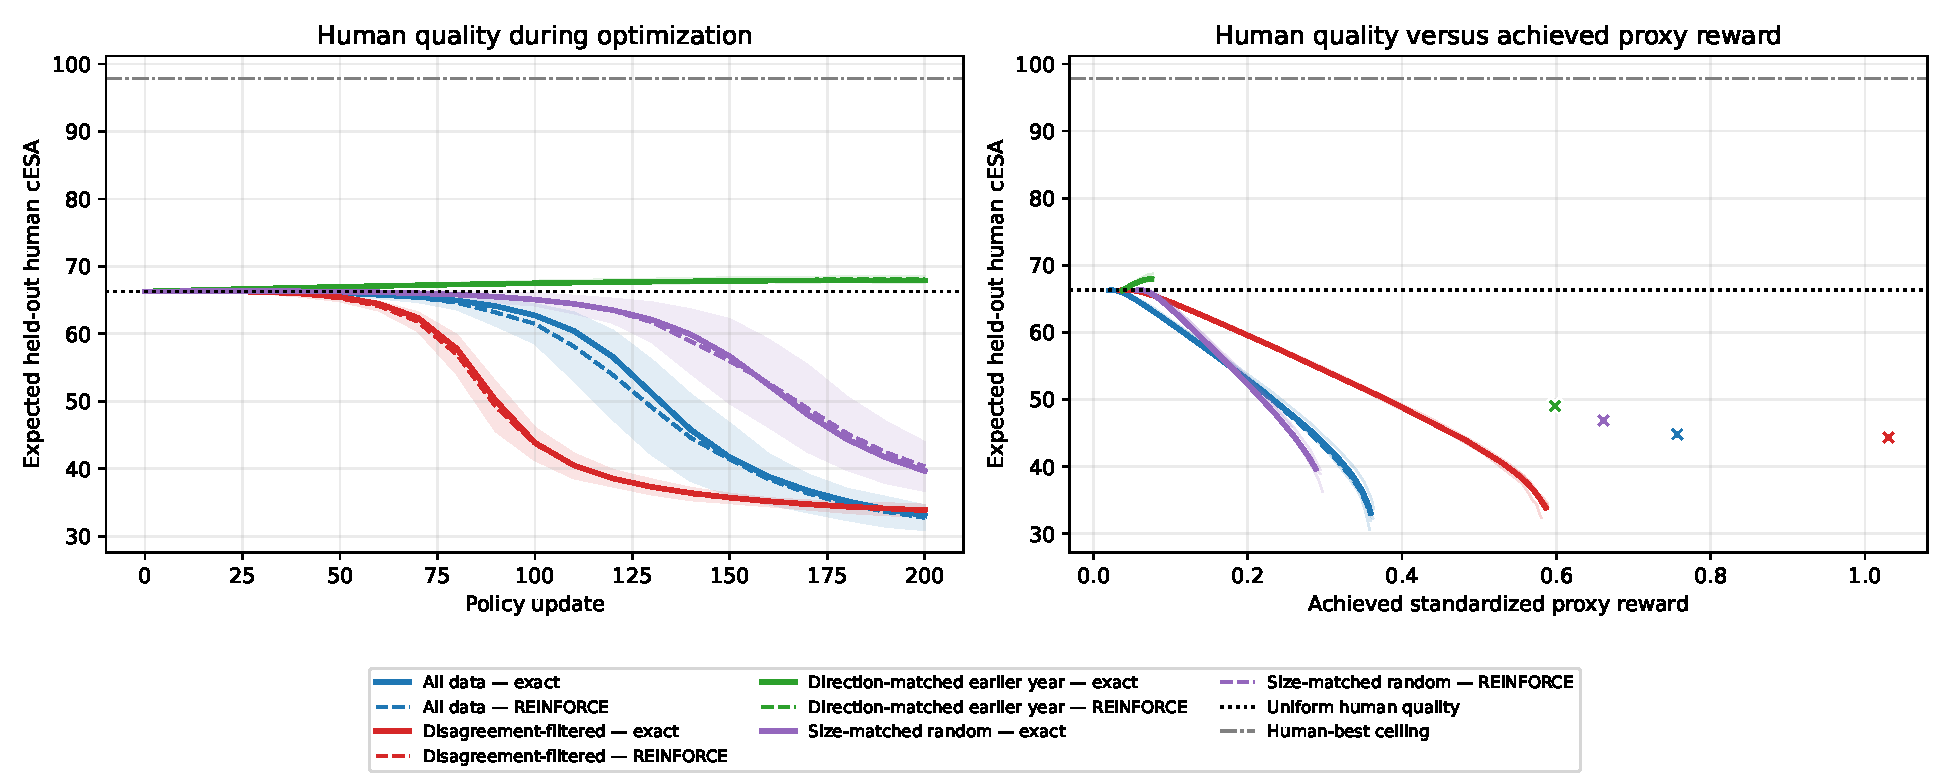
\includegraphics[width=\textwidth]{figures/contextual_bandit.pdf}
\caption{Held-out human cESA during policy optimization and against achieved
standardized proxy reward.  Solid lines are exact-gradient trajectories;
dashed lines average REINFORCE seeds, with shaded seed ranges.}
\label{fig:bandit}
\end{figure*}

\begin{table}[t]
\centering
\small
\setlength{\tabcolsep}{3pt}
\begin{tabular}{lrrr}
\toprule
Reward & Final cESA & $\Delta$ uniform & Interval \\
\midrule
All & \AllBanditCesa & \AllBanditChange & [\AllBanditLow, \AllBanditHigh] \\
Filtered & \FilteredBanditCesa & \FilteredBanditChange & [\FilteredBanditLow, \FilteredBanditHigh] \\
Random & \RandomBanditCesa & \RandomBanditChange & [\RandomBanditLow, \RandomBanditHigh] \\
Direction/year & \DirectionBanditCesa & \DirectionBanditChange & [\DirectionBanditLow, \DirectionBanditHigh] \\
\bottomrule
\end{tabular}
\caption{Exact-gradient expected held-out cESA after optimization.  Uniform
selection has cESA \UniformCesa{}; intervals use document-clustered bootstrap.}
\label{tab:bandit}
\end{table}

Three rewards learn policies far below uniform selection
(Table~\ref{tab:bandit}).  Their most probable action is the same system,
receiving mean probabilities \AllTopProbability{}, \FilteredTopProbability{},
and \RandomTopProbability{} under all-data, filtered, and random rewards.  The
direction-matched policy remains comparatively diffuse: its most probable
system receives \DirectionTopProbability{}.  The failure is therefore largely
system preference, not evidence that the source-conditioned policy discovered
useful translation routing.

\section{Discussion}

The study supports two conclusions.  First, modest development correlation
does not prevent substantial overoptimization under either best-of-$N$ or
policy gradients.  Second, reward-training composition matters: replacing
later into-English data with earlier slices produces qualitatively different
policy behavior.  What it does not show is equally important.  The diagnostic
flags dataset slices, not individual wrong labels; filtering does not reliably
beat matched removal; and one checkpoint per condition cannot separate a small
data effect from reward-training variability.

The bandit offers an exact RL test bed but cannot generate translations outside
its candidate pool.  Its fixed system actions also make system identity easy to
learn.  A stronger next experiment should score source--candidate text and hold
out complete systems, followed by multiple independently trained reward
checkpoints.  Generative RL would additionally require independent evaluation
of newly produced translations.

\section{Conclusion}

Optimizing learned MT rewards consistently exposes weaknesses that ordinary
development correlation obscures.  Metric--annotation disagreement is useful
for defining a targeted audit, but the present evidence does not validate it
as a filtering remedy.  The most robust finding is broader: label composition
can determine whether reward optimization mildly improves or catastrophically
reduces human-rated quality.

\section*{Limitations}

The diagnostic uses automatic metrics that overlap historically with some DA
training slices.  Matched controls cannot match system composition because the
source DA release omits system identifiers.  Holdouts differ in languages and
human protocols.  There is one reward-training seed per condition.  The
contextual policy selects among fixed systems and its test set is
source-disjoint, not an untouched confirmation set for the broader hypothesis.

\section*{Ethical Considerations}

This study reuses released WMT human judgments and candidate outputs.  It makes
no claim that individual annotators produced incorrect labels.  No new human
data were collected, and human outcomes were kept outside reward training and
policy optimization.

\bibliography{references}

\end{document}
